% !TeX encoding = UTF-8
\chapter{Allgemeine Bestimmungen für Abschlussarbeiten}
Die allgemeinen Bestimmungen für Studien- und Diplomarbeiten bzw. Bachelor- und Masterarbeiten regeln die für den jeweiligen
Studiengang geltenden Prüfungsordnungen (DPO, BPO bzw. MPO). Für den Fachbereich
Elektro- und Informationstechnik ist die jeweils Gültige auf den Internet Seiten des Fachbereichs
(\url{http://www.fb6.rwth-aachen.de/}) verfügbar. Dieses Merkblatt enthält
ergänzende Hinweise für die praktische Durchführung der Arbeit. Sollten Widersprüche zwischen diesem Dokument und der Prüfungsordnung bestehen, so gilt natürlich die Prüfungsordnung. Machen Sie sich unbedingt mit der für Sie geltenden Ordnung vertraut! Dies gilt speziell für Studierende anderer Fakultäten oder Universitäten.


\section{Bachelorarbeit}
Die Bachelorarbeit ist eine Prüfungsarbeit innerhalb der Fakultät, die die wissenschaftliche
Ausbildung zum Bachelor of Science abschließt. Neben der schriftlichen Ausarbeitung schließt
die Bachelorarbeit auch einen Vortrag über die Ergebnisse mit ein. 

Die Ausgabe des Themas erfolgt formal über die Vorsitzende bzw. den Vorsitzenden des
Prüfungsausschusses der Fakultät für Elektro- und Informationstechnik. Praktisch erfolgt die
Themenstellung der Bachelorarbeit von einem der Fakultät angeschlossenen Lehrstuhl. Die
Bearbeitungszeit für die Bachelorarbeit beträgt bei Vollzeitarbeiten drei Monate und bei Aufgaben die
in Teilzeit bearbeitet werden sechs Monate. Thema und
Aufgabenstellung müssen so beschaffen sein, dass die zur Bearbeitung vorgegebene Frist eingehalten
werden kann. Das Thema kann nur einmal und nur innerhalb des ersten Monats der
Bearbeitungszeit zurückgegeben werden. Im Einzelfall kann der Prüfungsausschuss auf begründeten
Antrag der Kandidatin bzw. des Kandidaten die Bearbeitungszeit ausnahmsweise um bis zu vier Wochen
verlängern. Die Arbeit inklusive Abschlussvortrag wird mit 12 CP bewertet.

Das Thema der Bachelorarbeit kann erst dann an den Bewerber oder die Bewerberin ausgegeben werden, wenn 120 CP erbracht wurden. 
Näheres regelt die jeweilige Bachelorprüfungsordnung. Zum Anfertigen einer Bachelorarbeit muss sich der Bewerber beim Zentralen
Prüfungsamt (ZPA) der RWTH anmelden.


\section{Masterarbeit}
Auszug aus der Master Prüfungsordnung \cite{MPO-10-2010}:
\begin{quote}
	\begin{enumerate}\setlength{\itemsep}{0pt}
		\setlength{\parsep}{0pt}
		\item Die Master-Arbeit besteht aus einer schriftlichen Arbeit der Kandidatin bzw. des Kandidaten.
		Sie soll zeigen, dass die Kandidatin bzw. der Kandidat in der Lage ist, ein Problem innerhalb
		einer vorgegebenen Frist nach wissenschaftlichen Methoden unter Anleitung selbstständig
		zu bearbeiten.
		\item Die Master-Arbeit kann von jeder bzw. jedem in Forschung und Lehre in der Fakultät für
		Elektrotechnik und Informationstechnik an der RWTH tätigen Professorin bzw. Professor
		ausgegeben und betreut werden. Lehrbeauftragte und wissenschaftliche Mitarbeiterinnen
		bzw. Mitarbeiter können bei der Betreuung mitwirken. In Ausnahmefällen kann die Master-
		Arbeit mit Zustimmung des Prüfungsausschusses außerhalb der Fakultät bzw. außerhalb
		der RWTH ausgeführt werden, wenn sie von einer der in Satz 1 genannten Personen betreut
		wird (s. Anlage 4).
		\item Auf besonderen Antrag der Kandidatin bzw. des Kandidaten sorgt die bzw. der Vorsitzende
		des Prüfungsausschusses dafür, dass sie bzw. er zum vorgesehenen Zeitpunkt das Thema
		einer Master-Arbeit erhält. Der Kandidatin bzw. dem Kandidaten ist Gelegenheit zu geben,
		für das Thema Vorschläge zu machen.
		\item Die Master-Arbeit kann im Einvernehmen mit der Prüferin bzw. dem Prüfer wahlweise in
		deutscher oder englischer Sprache abgefasst werden.
		\item Die bzw. der Vorsitzende des Prüfungsausschusses teilt der Kandidatin bzw. dem Kandidaten den Abgabetermin mit. Der Zeitpunkt der Ausgabe sowie die Themenstellung sind aktenkundig zu machen.
		\item Die Bearbeitungszeit für die Master-Arbeit beträgt maximal sechs Monate. Der Umfang der
		schriftlichen Ausarbeitung sollte ohne Anlage 80 Seiten nicht überschreiten. Das Thema kann nur einmal und nur innerhalb des ersten Monats der Bearbeitungszeit zurückgegeben
		werden. Ausnahmsweise kann der Prüfungsausschuss im Einzelfall auf begründeten Antrag
		der Kandidatin bzw. des Kandidaten und bei Befürwortung durch die Aufgabenstellerin bzw.
		den Aufgabensteller die Bearbeitungszeit um bis zu sechs Wochen verlängern.
		\item Die Ergebnisse der Master-Arbeit präsentiert die Kandidatin bzw. der Kandidat im Rahmen
		eines Master-Vortragskolloquiums.
	\end{enumerate}
\end{quote}


\section {Auswahl eines Themas}
Die üblicherweise ausgegebenen Themen können nach Schwerpunkten
unterteilt werden. Dies sind Arbeiten in
\begin{itemize}
	\item theoretischer Richtung (Modellbildung und Berechnungen, Simulation, Methoden)
	\item experimenteller Richtung (Meßtechnik, Messungen und Analyse der Messergebnisse)
	\item konstruktiver Richtung (Entwurf, Aufbau, Konstruktion)
\end{itemize}


Viele Arbeiten sind Teile der am Institut laufenden Forschungsarbeiten. Unter Umständen sind es
aber auch eigenständige Themen, wie z.B. Planung und Aufbau von Praktikumsversuchen oder besonderen
Geräten. Alle Arbeiten erfordern eine gewisse Einarbeitungszeit. Es wird empfohlen, die
Wahlvorlesungen rechtzeitig auch im Hinblick auf beabsichtigte Themenbereiche von Bachelor- und Masterarbeiten auszuwählen. Die Einarbeitung in ein bestimmtes 
Gebiet der Abschlussarbeit ist ein wesentlicher Bestandteil der selbständig durchzuführenden Arbeiten im Studium mit einem
meist besonders großen Lerneffekt. Es empfiehlt sich, frühzeitig ein methodisches Vorgehen zu
überlegen und in Absprache mit dem Betreuer einen Terminplan aufzustellen. Außerdem gehört ein
ausführliches Literaturstudium zur Einarbeitung. Die Auswahl des Themas selbst hängt weitgehend von den 
eigenen Interessen ab. Man sollte sich zuerst überlegen, welche Geräte oder Anlagen oder
welche theoretischen Methoden man gerne, auch im Hinblick auf den späteren Beruf, kennen lernen möchte. Dabei ist es empfehlenswert wenn die Themen von Bachelor- und Masterarbeit in verschiedenen Bereichen liegen,
um sich so in einem größeren "`Spektrum"' auszubilden. Diese Chance an der Universität sollte unbedingt genutzt werden.

\chapter{Durchführung der Arbeit}

\section{Beginn der Arbeit}
Als Termin für den Beginn der Arbeit gilt die Aushändigung der schriftlich formulierten Aufgabe.
Der Student erhält am Lehrstuhl notwendige Arbeitsmaterialien mit Ausnahme von Schreib- und
Zeichenmaterial. Ausgegebene Geräte dürfen nicht ohne Erlaubnis durch den Betreuer aus dem
Institutsbereich entfernt werden. Falls erforderlich, wird ein fester Arbeitsplatz zugewiesen. 


\section{Ablauf der Arbeit}
Zur eigenen Planung und Überwachung hat der Bearbeiter bei der Bachelor- und Studienarbeit spätestens 3 Wochen
bzw. bei der Master- und Diplomarbeit 6 Wochen nach Beginn der Arbeit ein Arbeitsprogramm und einen Terminplan
zu erstellen. Dieser ist mit dem betreuenden wissenschaftlichen Mitarbeiter abzusprechen. Bei einer
Masterarbeit folgt darauf der Einführungsvortrag (siehe Abschnitt~\ref{sec:vortrag}).

Während der gesamten Arbeit hat der Student einen ständigen Kontakt zu dem betreuenden wissenschaftlichen Mitarbeiter zu halten. Gesprächstermine (in der Regel wöchentlich) sind aus eigener Initiative des Studenten mit dem Betreuer zu vereinbaren.

\section{Der Einführungsvortrag\label{sec:vortrag}}
Der Einführungsvortrag sollte bei Masterarbeiten innerhalb der ersten 6 Wochen gehalten werden. 
In diesem Vortrag soll es nicht darum gehen schon möglichst viele fertige Ergebnisse zu präsentieren. Vielmehr geht es darum die kommende Arbeit zu strukturieren und ggf. erste Lösungsansätze zu präsentieren

Dazu soll mit eigenen Worten eine Einführung in die Themenstellung der Arbeit gegeben und die geplante Vorgehensweise mit Projektplan erläutert werden. Der Projektplan umfasst dabei
sowohl die \textbf{inhaltliche} (welche (Teil)-Ergebnisse sollen erreicht werden), die
\textbf{terminliche} (wann sollen die definierten Arbeitspakete abgeschlossen werden) und auch die
\textbf{finanzielle} (welche Investitionen sind erforderlich) Strukturierung der Arbeit. Der
Vortrag sollte einen Umfang von 10 Minuten haben und nicht mehr als 6 Folien enthalten.

\section{Bücher und Materialien}
Bücher, Materialien und Werkzeuge aus Institutsbeständen dürfen nicht aus den Räumen des Instituts entfernt werden, es sei
denn, ein Mitarbeiter hat dies explizit gestattet. In diesem Falle ist im  Sekretariat ein
Entleihschein zu hinterlegen. Die maximale Entleihzeit beträgt zwei Wochen. Danach sind die Sachen
umgehend an den betreuenden Assistenten zurückzugeben. Einige der am Lehrstuhl vorhandenen Dinge sind Privatbesitz (z.B. Bücher von Prof. Leonhardt). Diese dürfen nur nach expliziter Erlaubnis des Besitzers entliehen werden.

\section{Arbeitsende}
Bachelor-, Studien-, Master- und Diplomarbeiten sind von Studierenden der Fakultät für Elektrotechnik und Informationstechnik spätestens am letzten Tag des Bearbeitungszeitraums (siehe schriftliche Aufgabenstellung) im Sekretariat des Lehrstuhls abzugeben. Fällt dieser Termin auf ein Wochenende, einen Feiertag oder sonstige dienstfreie Tage, so gilt der nächste Arbeitstag als Abgabetermin. Informatiker oder Physiker geben ihre Diplomarbeiten im Zentralen Prüfungsamt ab. Machen Sie sich unabhängig von diesen Hinweisen mit den offiziellen Regelungen in Ihrer Fakultät vertraut.

\begin{figure}[!ht]
	\centering
	
\includegraphics[scale=0.6]{images/leimbindung}
	%% Reihenfolge der Befehle wichtig: zuerst die \caption, danach das \label
	\caption{Leimbindung}
	\label{fig:Leimbindung}
\end{figure}
Insgesamt sind bei der Abgabe zwei Exemplare der Arbeit in Leimbindung (siehe Abb.~\ref{fig:Leimbindung}) einzureichen. Von diesen muss eines das offizielle, unterschriebene und im Sekretariat bereitliegende Deckblatt als vorderste Seite verwenden.
Umfangreichere Anhänge, die nicht zusammen mit dem Hauptteil der Arbeit gebunden werden können, müssen nicht unbedingt in einer Leimbindung eingereicht werden; hier kann auch ein Leitz-Ordner (feste Struktur, weißes Rückenschild) verwendet werden.
Der Druck der Arbeit kann in Graustufen (Schwarzweiss) oder Farbe erfolgen. Im Fall des Schwarzweissdrucks müssen Grafiken derart gestaltet sein, dass alle Informationen ohne Farbe erkennbar sind.


Von allen Texten, Bildern, Programmen, Messdaten, Vorträgen und sonstigen im Rahmen der Arbeit entstandenen Daten muss eine Sicherungskopie auf einem
archivierbaren Datenträger (z.B. CD, DVD) erstellt und in jede Arbeit eingelegt
werden. Zusätzlich muss die schriftliche Arbeit in elektronischer Form als Postscript- und
PDF-Datei sowie im Original-Erstellungsformat (\LaTeX\ , Word, etc...) abgegeben werden. Die Kosten, die bei der Herstellung der Abgabeexemplare anfallen (Kopien/Binden/etc...), gehen im Regelfall zu Lasten des Studenten. Bei Abschluss der Arbeit sind alle Geräte, Bücher, Schlüssel u.ä. zurückzugeben. Erst nach erfolgter Rückgabe der genannten Materialen, der Übergabe des Datenträgers und der Präsentation des abschließenden Seminarvortrags kann die Note in die Prüfungsakte eingetragen werden. Bei Bachelor- und Masterarbeiten wird das Datum der Abgabe der schriftlichen Ausarbeitung in die Prüfungsakte eingetragen, nicht das Datum des evtl. späteren Seminarvortrags.

Nach Abgabe der schriftlichen Arbeit kann bei Bedarf durch den Lehrstuhl eine sogenannte ''4.0 Bescheinigung'' ausgestellt werden.

\section{Abschlussvortrag}

Über die angefertigte Arbeit ist ein Vortrag von typischerweise 15 Minuten (Bachelorarbeit) / 20 Minuten (Masterarbeit) in möglichst freier Rede
zu halten. 
Der Vortrag findet im MedIt Doktorandenseminar statt, Gäste sind zugelassen. Es ist ratsam den Vortragstermin frühzeitig festzulegen und in der Tagesordnung einen Platz zu reservieren. 


Der Vortrag soll sich an ein sachkundiges Publikum ohne Spezialkenntnisse wenden. Er
muss daher vor allem die Problemstellung, den Lösungsansatz und die Ergebnisse klar darlegen,
braucht aber nur wenige Detailinformationen zu enthalten. Es soll hier eine Darstellung der Aufgabe
oder auch nur eines Teilbereichs der Aufgabe, aber kein Tätigkeitsbericht geboten werden. Ein
einziges gut ausgearbeitetes Beispiel kann oft mehr zeigen als eine große Anzahl von Fakten, die
wegen der gedrängten Information vom Zuhörerkreis in der kurzen Zeit nicht verstanden werden
können.

Im Anschluss an den Vortrag können Geräte und Versuche dem Zuhörerkreis vorgeführt werden.

Die Gliederung ist zu Beginn des Vortrags anzugeben und in kurzer Form zu erläutern. Während des
Ablaufs soll zur Orientierungshilfe immer auf den behandelten Gliederungspunkt hingewiesen werden.

Wie erwähnt soll der Vortrag insgesamt 15/20 Minuten dauern. Zur Abschätzung der Vortragsdauer kann
man ungefähr 1 - 2 Minuten zur Erläuterung einer beschriebenen Folie ansetzen. Der gesamte Vortrag
sollte somit nicht mehr als 12 Folien umfassen (inklusive Titel und Gliederung).

Im allgemeinen erfolgt die Darstellung als elektronische Präsentation auf den Computer. Zur Erstellung von Vortragsfolien existieren eine Reihe verschiedener Programme, wie z.B. Microsoft
Powerpoint, Libre Office, aber auch mit \LaTeX\  erzeugte Postscript und PDF Dokumente können für
einen Vortrag genutzt werden. Eine Designvorlage für Powerpoint und \LaTeX\  wird vom Institut zur Verfügung gestellt.

Bei der Darstellung ist darauf zu achten, dass die verwendeten Schriften 16pt nicht unterschreiten.
An sämtlichen Diagrammen sind die dargestellten Größen mit Wort, Zeichen und Dimension anzugeben.
Multimedia Effekte (wie z.B. Ton oder Videos) können richtig angewendet große Wirkung erzielen,
allerdings nur, wenn sie der Darstellung von Information dienen. Auch die Animation von Grafiken
und Schrift sollte so sparsam wie möglich eingesetzt werden. Bei der Auswahl von Farben (z.B. für
Schriften, Hintergrund und Hervorhebung) sollte darauf geachtet werden, nicht zu viele verschiedene
Typen zu verwenden. Hilfe gibt auch hier die Folienvorlage des Instituts.

Bei der Gestaltung der Folien empfiehlt sich die Verwendung von Bildern anstelle langer
zusammenhängender Textpassagen:
\begin{quote}\rmfamily\small\itshape
	"`Ein Bild sagt mehr als 1000 Worte"'
\end{quote}

\paragraph{Probevortrag}
Es empfiehlt sich, den Vortrag mehrfach probeweise zu Hause (und evtl. vor dem Betreuer) zu halten
und dabei laut zu sprechen. Anfangs wird die Dauer noch mehr als doppelt so lange sein, mit
flüssigerem Vortrag soll dann aber die angestrebte Vortragsdauer erreicht werden. Anfangs empfiehlt
es sich auch zu jeder Folie einige Stichpunkte auf einen Handzettel zu notieren, an denen man sich
während des Vortrags orientieren kann.


\chapter{Abfassung der schriftlichen Arbeit}
Als Ergebnis der Arbeit ist ein schriftlicher Bericht
vorzulegen. Dieser Bericht soll für einen unvorbereiteten, aber fachkundigen Leser leicht
verständlich sein. Dabei ist auch von möglichst kompakten Formulierungen und Darstellungen Gebrauch
zu machen. Für die Länge der schriftlichen Ausarbeitung sind bei einer Bachelorarbeit etwa 50 Seiten und bei einer Masterarbeit ca. 70 Seiten (ohne Anhang) anzustreben. Dies sind natürlich nur Richtwerte, aber eine deutlich längere Arbeit (ohne dass der Inhaltliche 
Gehalt dies erfordert) wird nicht zwangsläufig besser beurteilt. Hingegen wird eine kürzere auch nicht schlechter bewertet, wenn dafür auf verlängernde Prosa verzichtet wird.

Es wird empfohlen, den Text der Arbeit unter Verwendung gängiger Textverarbeitungsprogramme auf
weißes Papier DIN A4 zu schreiben. Der Ränder sollten umlaufend mindestens 2,5 cm breit sein und es
sollte eine 1 bis 1,2-zeilige Schreibweise in 12pt Schrift gewählt werden. Als \LaTeX\ Vorlage kann der Quelltextes des vorliegenden Dokumentes verwendet werden.

\section{Titelbild}
Die Richtlinien zur Verwendung von Logos sind in der RWTH kompliziert geregelt. Das hat in der Vergangenheit immer wieder zu Problemen geführt. Darum haben wir bewusst auf das MedIT Logo und das RWTH Logo verzichtet. 

Vielmehr sollte das Titelbild die ganze Aufmerksamkeit erhalten und Interesse für den Inhalt der Abschlussarbeit wecken.



\section{Eidesstattliche Versicherung}\label{sec:eidesstattlich}
Bei jeder wissenschaftlichen Arbeit zum Zwecke der Erlangung einer formalen Qualifikation ist eine eidesstattliche Versicherung abzugeben.
Der von der RWTH Aachen dafür vorgegebene Vordruck für diese Erklärung ist bereits in der \LaTeX\ Vorlage für dieses Dokument enthalten.

In diesem Zusammenhang sei empfohlen, den Text der Erklärung einmal genau zu lesen. Eine Eidesstattliche Versicherung ist eine Ernst zu nehmende Angelegenheit und kann schwerwiegende Konsequenzen haben, z.B. im schlimmsten Falle die Aberkennung der Prüfungsleistung.

Die verwendeten Hilfsmittel bei der Erstellung der Arbeit sind in Anhang \ref{sec:AnhangHilfsmittel} aufzulisten
\clearpage

\section{Gliederung der Arbeit\label{sec:kap_seiten}}
Typischerweise enthält eine wissenschaftliche Arbeit die im folgenden aufgeführten Abschnitte:

\begin{tabular}{lcll}
	Aufgabenstellung (wird vom Institut erstellt)   &\hspace{3cm} & &\\
	Erklärung der Selbständigkeit &&&\\
	Zusammenfassung &  & &i \\
	Inhaltsverzeichnis & && ii\\
	Verwendete Symbole& & &iv\\
	\\
	1. Einführung & &Seite& 1 \\
	2. Grundlagen&&& 3 (z.B.)\\
	\hspace{5mm} 2.1 & & &.       \\
	\hspace{10mm} 2.1.1& & &. \\
	\hspace{10mm} 2.1.2& & &.\\
	\hspace{20mm} a)\\
	\hspace{20mm} b)\\
	\hspace{5mm} 2.2& & &.\\
	\hspace{5mm} 2.3& & &.\\
	.\\
	.\\
	5. Ergebnisse& & &.\\
	6. Zusammenfassung und Ausblick&&& 60 (z.B.)\\
	Literaturverzeichnis &&&63\\
	Tabellenverzeichnis (optional)\\
	Bilderverzeichnis (optional)\\
	Anhang\\
	A\\
	B\\
	.\\
	.\\
\end{tabular}


Die Aufteilung der Abschnitte sollte so gewählt werden, dass alle inhaltlichen Abschnitte (also
Grundlagen bis Ergebnisse) in etwa den gleichen Seitenumfang haben und nicht weniger als 15 Seiten
umfassen. Die Untergliederung sollte nicht übertrieben werden. In der Regel ist eine Aufgliederung
bis in die dritte Ebene (z.B. 2.1.1) hinreichend.




\section{Zusammenfassung}
Am Anfang der Arbeit steht eine kurze Zusammenfassung mit einer maximalen Länge von einer
halben Seite. Darunter sind bis zu fünf Schlüsselwörter für die Arbeit anzugeben. Wenn
möglich, ist die Zusammenfassung ("`abstract"') zusätzlich auch in englischer Sprache anzugeben.

\section{Inhaltsverzeichnis}
Das Inhaltsverzeichnis soll entsprechend DIN 1421 in gestaffelter Dezimalgliederung mit
arabischen Ziffern aufgestellt werden und die zu den Abschnitten gehörigen Seitenangabe
enthalten. Als Beispiel kann das Inhaltsverzeichnis dieses Dokumentes herangezogen werden.
Die einleitenden Seiten wie Titelseite, Aufgabenstellung, Danksagung, Erklärung der selbstständigen Anfertigung, Abstract und die Verzeichnisse (z.B. Symbol-, Inhalts- und Tabellenverzeichniss) werden separat mit kleinen römischen Ziffern nummeriert. Die erste Seite mit der arabischen Seitennummer 1 ist die Einführung (vgl. Abschnitt~\ref{sec:kap_seiten} und das Inhaltsverzeichnis dieses Dokuments).


\section{Verzeichnis der verwendeten Symbole und Abkürzungen}

Die wesentlichen in der Arbeit verwendeten Symbole und Abkürzungen sind in einer Liste nach dem
Inhaltsverzeichnis aufzuführen. Die Verwendung der Symbole soll sich, wenn möglich, an die für das
behandelte Fachgebiet herausgegebenen Normen und Richtlinien anlehnen und ist jeweils mit dem
Betreuer abzusprechen. Die jeweiligen Dimensionen sind hinzuzufügen. Ein Beispiel gibt nachfolgende
Tabelle:

\begin{table}[!ht]
	\centering
	\vspace{5mm}
	%% Reihenfolge der Befehle wichtig: zuerst die \caption, danach das \label
	\captionabove{Beispiel der Angabe von Symbolen}
	\begin{tabular}{|ll|}
		\hline
		p & Formelsymbol für Druck in [Pa],[$\,$mm$\,$Hg] oder [cm$\,$H$_2$O]\\
		$\dot V$ & Volumenstrom in [ml/h],[ml/min], [ml/sek], definiert als dV/dt\\
		\hline
	\end{tabular}
	
	\label{tab:AngabeVonSymbolen}
\end{table}
Es sind, soweit es möglich ist, die internationalen SI-Einheiten zu verwenden.

\section{Einleitung}
In der Einleitung soll in die behandelte Problemstellung kurz eingeführt werden. Weiterhin
sollen Bezüge zu anderen Arbeiten, der wissenschaftliche Hintergrund und der Stand des
Wissens und der Technik sowie die Motivation und Zielsetzung der Arbeit aufgezeigt werden.

\section{Textteil}
\subsection{Formale Gestaltung}
Die Seiten der Arbeit sind fortlaufend zu nummerieren. Bilder und Tabellen sollen abschnittsweise
durchnummeriert werden (z.B. \figurename~2.1, \figurename~2.2, \figurename~2.3,\ldots\ , \figurename~5.1, \figurename~5.2,...). Einheitlich
ist nur die Bezeichnung "`\figurename"' zu verwenden. Andere Bezeichnungen sind zu vermeiden. Unter jeder Abbildung muss eine Legende mit einer kurzen, erläuternden Beschreibung
vorgesehen werden. Auf alle Bilder und Tabellen ist im Text mindestens einmal zu verweisen (z.B.
"`\ldots\  wie in \figurename~\ref{fig:beispiel1} zu sehen"'). Werden Bilder aus fremden Quellen (z.B. Büchern,
Software, Bildersammlungen, Internet, etc...) verwendet, so ist die Quelle  anzugeben, siehe
Unterschrift \figurename~\ref{fig:beispiel1}. In Diagrammen sind Sämtliche Achsen und Kurven mit
aufgetragener Größe und Einheit zu beschriften. Bitte darauf achten, dass die Schriftgröße bei nachträglicher Skalierung sowohl lesbar ist als auch nicht zu groß wird. Als Richtwert sollte keine Beschriftung kleiner als 8pt und größer als 16pt in der finalen Ausgabe erscheinen.

\begin{figure}[!ht]
	\centering
	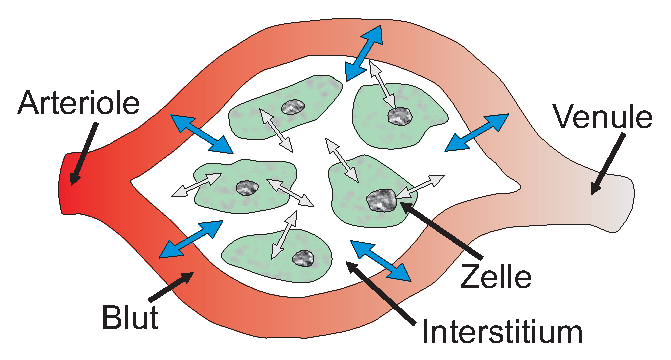
\includegraphics[scale=.65]{images/beispiel1}
	\hspace{8mm}
	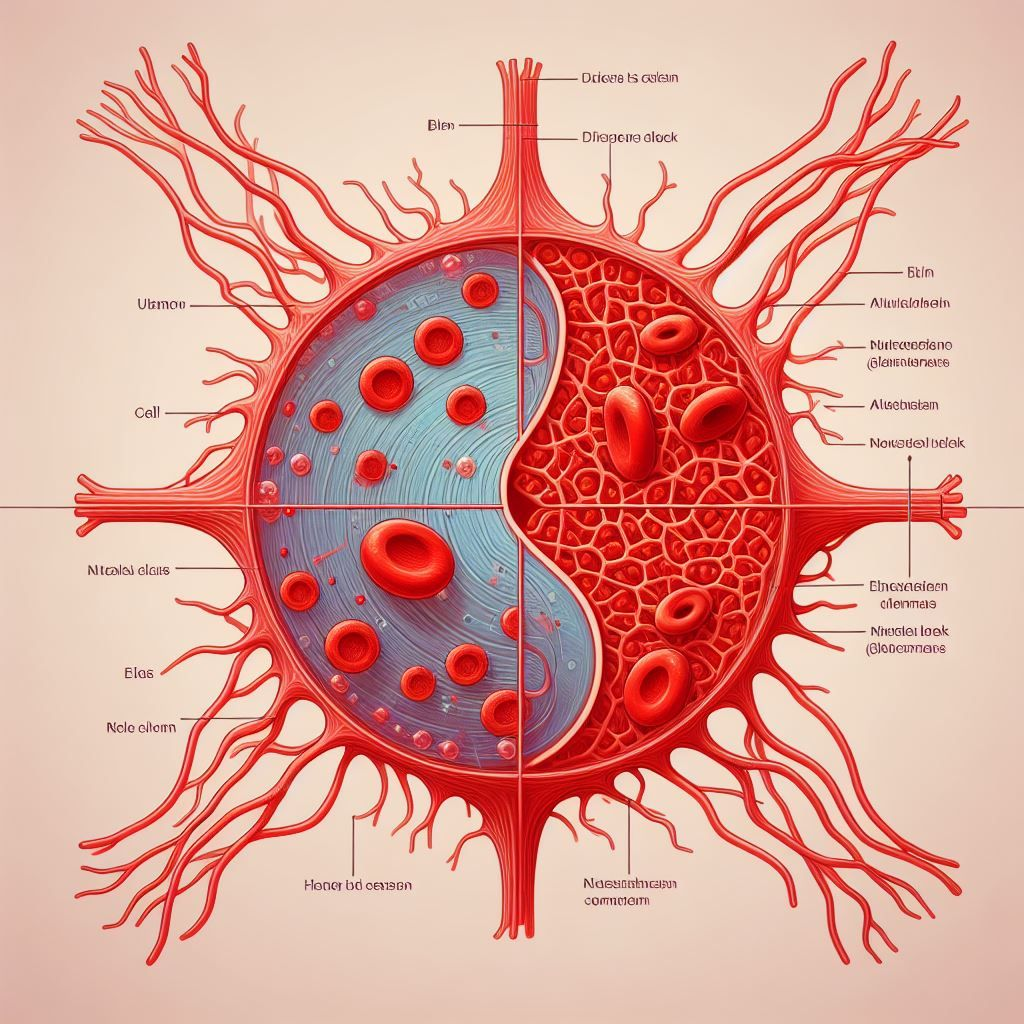
\includegraphics[width=5cm]{images/AI_cell_picture}
	% Die folgende Anweisungen bindet die Grafik nocheinmal zusätzlich
	% als Dateianhang ein. Das hat den Vorteil, dass sie einfach aus dem pdf zur
	% wieterverwendung extrahierbar ist und der Autor (author) mit angegeben
	% werden kann. Leider ist die Grafik dadurch auch gleich zweimal im pdf
	% enthalten und verbraucht dadurch doppelt Platz.
	% \textattachfile[mimetype=application/pdf,print=false,author=\docauthor,description=\figurename~\ref{fig:beispiel1}]{beispiel1.pdf}{}
	%% Reihenfolge der Befehle wichtig: zuerst die \caption, danach das \label
	\caption{Der Gasaustausch zwischen Blut und Zellen findet auf kapillarer Ebene über das Interstitium statt, links aus \cite{walter2002}}
	\label{fig:beispiel1}
\end{figure}


Gleichungen werden zentriert und am rechten Rand abschnittsweise nummeriert(z.B. (2.1), (2.2),...; (5.1),
(5.2),...). Ein Beispiel gibt nachfolgende Gl.~(\ref{eqn:e_mod_laminar}).
\begin{equation}\label{eqn:e_mod_laminar}
	\dot V = \frac{\pi \, \Delta p \, r^4}{8 \, \eta \, l} =
	G_{Strom} \: \Delta p
\end{equation}

\begin{equation}\label{erster}
	\begin{split}
		a &= b +c \\
		&= e + f
	\end{split}
\end{equation}
Man beachte: Bilder haben Bildunterschriften, Tabellen haben Tabellenüberschriften, siehe
\tablename~\ref{tab:beispiel}. Die neuen amtlichen Regeln und Schreibungen der deutschen
Rechtschreibung sind zu beachten.

\begin{table}[!ht]
	\centering
	%% Reihenfolge der Befehle wichtig: zuerst die \caption, danach das \label
	\captionabove{Dies ist eine Tabellenüberschrift}
	\begin{tabular}{l|cr}
		Spalte 1 & Spalte 2 & Spalte 3\\
		\hhline{|=|==|}
		Links & Mitte & Rechts\\
		\hhline{---}
		eins & zwei & drei
	\end{tabular}
	\label{tab:beispiel}
\end{table}

Auf alle Bilder, Tabellen und Gleichungen ist im Text mindestens einmal zu verweisen (z.B. ... wie
man in \figurename~\ref{fig:beispiel1} erkennt, ....). Die Platzierung der Bilder und Tabellen soll in
unmittelbarer Nähe zu diesem (ersten) Textverweis erfolgen.


\subsection{Grundlagen / Stand der Technik}
In einem besonderen Abschnitt sollen die notwendigen theoretischen und praktischen Grundlagen
und Voraussetzungen der Arbeit dargestellt werden. Auf Beweise, ausführliche Ableitungen und
weitergehende Erläuterungen kann, soweit sie in der Literatur bekannt sind, verzichtet werden.
Umfangreiche Zwischenrechnungen und nebensächliche Ausarbeitungen sollen im Anhang
untergebracht werden.

\subsection{Durchführung}
In den folgenden Abschnitten sollen die Ergebnisse der Arbeit dargestellt werden. Dabei soll insbesondere
erkennbar sein, was selbst erarbeitet und was evtl. aus welcher anderen Arbeit (Zitat) unmittelbar
entnommen und in die eigene Arbeit integriert wurde. Eine genaue Beschreibung der
erstellten Berechnungen, Programme, Schaltungen oder Konstruktionen und ähnlichem ist
erforderlich. Alle notwendigen Bilder (z.B. in Form von Plänen, Diagrammen) und sonstige
Unterlagen sind, soweit sie zur Erläuterung benötigt werden, hier einzufügen.

\subsection{Dokumentation von Software}
Die Beschreibung muss so erstellt sein, dass ein späterer Benutzer das Programm für sein Problem
leicht einsetzen bzw. die für ihn notwendigen Änderungen durchführen kann. Sie beinhaltet eine
Darstellung der Aufgabe und des Aufbaus des Programmsystems sowie eine Beschreibung der verwendeten
Unterprogramme. Hierbei können beispielsweise Ablaufdiagramme oder Psudocode für die Erklärung
sinnvoll verwendet werden. Bei umfangreichen Softwarepaketen mit einem User-Interface kann es
sinnvoll sein, zusätzlich eine kurze Bedienungsanleitung zu erstellen, die die Verwendung erklärt.
Ein Abdruck des gesamten Programmcodes ist nicht notwendig.

Bei der Darstellung des Programmsystems soll ein Überblick über die Aufgabe und den Ablauf des
Gesamtsystems gegeben werden. Die Organisation und die Verknüpfung der Komponenten muss erläutert
werden. Die notwendigen Ein- und Ausgaben, die Bedeutung der Parameter und evtl. vorhandene
Steuermöglichkeiten sollen angegeben werden. Oftmals ist es sinnvoll auch die grundsätzlichen
Ideen, Überlegungen und Randbedingungen, die zu der verwendeten Implementierung geführt haben zu
dokumentieren.

Ein wesentlicher Teil der Softwaredokumentation erfolgt durch Kommentare im Programmtext selbst. So
ist jede Komponente mit einem Header zu versehen, der die verwendeten Ein- und Ausgangsgrößen (in
Format, Wertebereich und Bedeutung), die benutzten und ggf. veränderten globalen Variablen, und
eine kurze und prägnante Beschreibung der Arbeitsweise enthält. Auch im weiteren Verlauf sind
Kommentare möglichst oft für die weitere Erklärung der Funktion zu verwenden.


\subsection{Dokumentation von Schaltungen}
Schaltungen von elektrischen Geräten werden am günstigsten zuerst in einem Blockschaltbild
dargestellt. Die Arbeitsweise von einzelnen, nicht allgemein gebräuchlichen Schaltungsarten sollte
bei der Beschreibung der Gesamtschaltung besonders hervorgehoben werden. Besonderes Augenmerk ist
auf die Einstell- und Abgleichvorschriften zu legen, um einem späteren Benutzer die Verwendung zu
erleichtern. Auch Prüfvorschriften zur Ermittlung von Fehlern bzw. defekten Bauteilen sind
anzugeben. Im Anhang sind eine vollständige Bauteileliste (inkl. Bezugsquellen), die
Schaltungsauslegungen mit evtl. vorhandenen Layouts für gedruckte Platinen, Bestückungszeichnungen
und Steckerbelegungspläne anzugeben. Von wenig gebräuchlichen Einzelkomponenten (z.B. Spezial-IC's)
sollten relevante Auszüge der Datenblätter in den Anhang eingefügt werden.

\subsection{Dokumentation von mechanischen Konstruktionen}
Mechanische Aufbauten sollten in der Arbeit selbst durch Prinzipskizzen nach den Regeln technischer
Zeichnungen (DIN Taschenbuch 2, Normen technisches Zeichnen \cite{DIN_Norm_TZ}) und Fotos
dargestellt werden. Besonderheiten bei der Anfertigung, wie spezielle Fertigungsverfahren,
Zusammenbau und Justiervorschriften, sind gesondert zu erläutern. Im Anhang sollen maßstabsgetreue
Einzelteilzeichnungen und Zusammenbauzeichnungen beigefügt werden. Falls die Durchführung von
Wartungsarbeiten erforderlich ist, muss ein entsprechender Maßnahmenkatalog enthalten sein.

\subsection{Ergebnisse\label{sec:ergebnisse}}
Im vorletzten Abschnitt sollen die bei der Durchführung der Arbeit gewonnenen Ergebnisse
zusammengefasst dargestellt werden. Besonders wichtig ist eine Wertung und Einordnung der
Ergebnisse. Auch Nicht-Erfolge können ein Ergebnis sein. Messkurven und Messreihen gehören, solange
sie nicht als Beispiel ein spezielles Ergebnis erläutern, in den Anhang.

\subsection{Zusammenfassung und Ausblick}
Neben einer kurzen Zusammenfassung der wichtigsten Ergebnisse soll in diesem Abschnitt auf
weiterführende Fragestellungen oder noch offene, durch die Arbeit aufgeworfene, Probleme
hingewiesen werden (Umfang maximal 2-3 Seiten).


\section{Umgang mit geistigem Eigentum Dritter}

Nicht zuletzt durch die öffentliche Diskussion um die Dissertationen einiger Politiker ist das Thema Plagiat und Urheberschaft in der wissenschaftlichen Praxis in den Fokus des Interesses gerückt. Hierbei müssen zwei Rechtsaspekte voneinander unterschieden werden. Zum einen das Urheberrecht. Hier geht es darum, dass ein Autor bestimmte Rechte an seinem Werk hat und somit bestimmte Bedingungen bei der Publikation eingehalten werden müssen, damit die Rechte des Autors nicht verletzt werden.
Der andere Aspekt betrifft die geistige Urheberschaft originärer Gedanken. Hier geht es in der wissenschaftlichen Praxis darum kenntlich zu machen, wer der geistige Urheber des geschriebenen Textes ist und welches Maß an eigener Leistung darin enthalten ist. Nicht zuletzt bei wissenschaftlichen Arbeiten ist dies ja auch ein relevantes Bewertungskriterium. 

Aber nicht nur Doktorarbeiten prominenter Politiker unterliegen diesen Rechtsnormen, auch eine studentische Abschlussarbeit hat die gleichen Anforderungen zu erfüllen. Dies wird nicht zuletzt auch durch die eigene Unterschrift unter die Eidesstattliche Versicherung in dieser Arbeit selbst nochmals bestätigt.


Die Frage von Lizenzen für urheberrechtlich geschütztes Material findet in der Abschlussarbeit üblicherweise keine Anwendung da das Ergebnis der Bachelor- oder Masterarbeit ja nicht öffentlich publiziert wird und damit nach deutschem Urheberrecht die freie Verwendung gestattet ist. Die Frage der geistigen Urheberschaft ist aber in jedem Falle zu beachten (Zitatregeln nicht vergessen!).

Zur Überprüfung der Einhaltung der Rechtsnormen gehen immer mehr Universitäten dazu über, alle Abschlussarbeiten einem automatischen Plagiats-Check durch entsprechende Software zu unterwerfen. An der RWTH Aachen ist dies derzeit nicht verpflichtend, aber erste Pilotprojekte wurden gestartet. Zudem ist auch zu bedenken, dass selbst wenn ein solcher Check heute noch nicht stattfindet, es nicht auszuschließen ist, dass dieser irgendwann in der Zukunft nicht auch retrospektiv durchgeführt wird und damit dann schlimmstenfalls die schon längst abgeschlossen geglaubte Prüfungsleistung in Gefahr gerät.

Weitere Informationen zum Thema können beispielsweise in \cite{deutsche_forschungsgemeinschaft_2022_6472827}, \cite{Uni_Wien} und \cite{Unijournal06_4} gefunden werden. 


\subsection{Literaturzitate}
Bei der Abhandlung einer wissenschaftlichen Arbeit steht man also vor einem Dilemma, dass einerseits gerade das Studium und die Aufarbeitung der Literatur ja ein zentrales Werkzeug der wissenschaftlichen Arbeit ist, andererseits im Text klar kenntlich werden soll, was eine eigene Leistung und was der Anteil Dritter am Ergebnis ist. Hierbei ist es wichtig festzustellen, dass es keineswegs eine Abwertung bedeutet, wenn Quellen Dritter im eigenen Text verwendet werden, vielmehr macht es im Gegenteil deutlich, dass der Autor mit der Materie vertraut ist und den Stand der Technik gut überblickt. Behauptungen und Fakten, die im Weiteren Verlauf der Arbeit nicht abgeleitet, ermittelt oder bewiesen werden, sollten durch einen Quellenverweis (sog. Belegzitat) ausgestattet werden.

\begin{quote}
	... zur Bestimmung der Ordnung eines ARMA Signalfilters kann das sogenannte ''Akaike Information Criterion'' \cite{Akaike1974a} herangezogen werden.
\end{quote}

Davon ausgenommen ist die Beschreibung von Grundlagenwissen, das bei der typischen Leserschaft als bekannt vorausgesetzt werden kann. Dafür stelle man sich beispielsweise einfach vor, was ein durchschnittlicher Fachstudienkollege wissen würde, der keine Abschlussarbeit direkt im gleichen Thema geschrieben hat.

Bei jeder wissenschaftlichen Arbeit wird besonderer Wert auf die vollständige und einheitliche Zitierung fremder Quellen gelegt. Vollständigkeit bedeutet, dass jede Verwendung fremden geistigen Eigentums durch genaue Quellenangabe kenntlich gemacht werden muss. Es ist hierbei zu unterscheiden
zwischen der wörtlichen, der genauen inhaltlichen und der sinngemäßen Wiedergabe. Der wörtlich übernommene Text (Sätze, Satzteile, einzelne Wörter) ist durch Anführungszeichen ("`die Axt im \ldots\  erspart den Zimmermann"', aus \cite{Schiller:Tell}) zu kennzeichnen. Dabei darf der Text nicht
verändert werden. Die Auslassung eines oder mehrerer Worte ist durch drei Punkte (\ldots\ ) anzudeuten. Es ist immer der Ursprungstext zu zitieren, nicht etwa das Zitat durch einen anderen (Primärzitate statt Sekundärzitate verwenden). Nur, wenn das Original nicht beschaffbar ist, sollte man hiervon Gebrauch machen. Dann ist aber die Sekundärliteratur zu referenzieren und auf das Zitat (z.B. zit. nach ...) hinzuweisen.

\begin{quote}\rmfamily\small\itshape
	Lange Zitate können zusätzlich durch eingerückten engeren Schriftsatz mit kleinerer, kursiver Schrift (wie mit diesem Satz angedeutet) abgehoben werden.\end{quote}

Werden fremdsprachige Texte in eigener Übersetzung wiedergegeben, so ist dies kenntlich zu machen
("`\ldots\  Text \ldots\ "' Übersetzung aus \cite{Akaike1974a}). Auch die genaue inhaltliche oder die sinngemäße Wiedergabe fremden geistigen Eigentums ist durch unmissverständlichen Quellenverweis kenntlich zu machen.

Die Anwendung der Zitatregeln soll an folgendem Beispiel aus \cite{web_pruschmann} deutlich werden:

\begin{quote}\rmfamily\small\itshape
	Mit Hilfe einer Textstelle aus der Publikation ''Geschlecht. Wider die Natürlichkeit'' von Heinz-Jürgen Voß soll verdeutlicht werden, was gemeint ist:
	
	Das Originalzitat: ''Gegen solche ''darwinistischen Schwärmereien'' der Entwicklung auch von Frauengehirnen auf ähnliche oder gleiche Höhe wie die der Männer, wenn es die gesellschaftlichen Bedingungen endlich zuließen, regte sich Widerstand, so bei Paul Julius Möbius, der sich energisch gegen die Frauenemanzipation wandte.'' \cite{Voss2011},S. 211
	
	Verwendungsbeispiel 1: Gegen solche ''darwinistischen Schwärmereien'' der Entwicklung auch von Frauengehirnen auf ähnliche oder gleiche Höhe wie die der Männer, wenn es die gesellschaftlichen Bedingungen endlich zuließen, regte sich Widerstand, so bei Paul Julius Möbius, der sich energisch gegen die Frauenemanzipation wandte. (Ein klares Plagiat. Es fehlen die Anführungszeichen und die Quellenangabe.)
	
	
	Verwendungsbeispiel 2: Gegen solche ''darwinistischen Schwärmereien'' der Entwicklung auch von Frauengehirnen auf ähnliche oder gleiche Höhe wie die der Männer, wenn es die gesellschaftlichen Bedingungen endlich zuließen, regte sich Widerstand, so bei Paul Julius Möbius, der sich energisch gegen die Frauenemanzipation wandte \cite{Voss2011},S. 211. (Die Quelle wird zwar angegeben, aber die Textpassage wird nicht durch Anführungszeichen als Zitat gekennzeichnet. Es handelt sich ebenso um ein Plagiat.)
	
	Verwendungsbeispiel 3: Gegen solche ''darwinistischen Schwärmereien'' der Entwicklung von Frauengehirnen auf ähnliche Höhe wie bei Männern, wenn es die gesellschaftlichen Bedingungen zuließen, regte sich zum Beispiel bei Paul Julius Möbius Widerstand, der sich entschieden gegen die Frauenemanzipation wandte \cite{Voss2011},S. 211. (Das ist ebenso ein Plagiat. Das Zitat wurde nur geringfügig abgeändert, doch es ist noch keine Paraphrase und die übernommenen Formulierungen müssen als Zitat gekennzeichnet werden. Durch das leichte Redigieren der Textstelle entsteht hier sogar der Verdacht einer bewussten Täuschung. Diese Vorgehensweise wird auch Verteidigungsminister zu Guttenberg vorgeworfen.)
	
	Verwendungsbeispiel 4: ''Gegen solche 'darwinistischen Schwärmereien' der Entwicklung auch von Frauengehirnen auf ähnliche oder gleiche Höhe wie die der Männer, wenn es die gesellschaftlichen Bedingungen endlich zuließen, regte sich Widerstand, so bei Paul Julius Möbius, der sich energisch gegen die Frauenemanzipation wandte.'' \cite{Voss2011},S. 211. (Hier wird die übernommene Textstelle korrekt ausgewiesen (Ausführungszeichen) und die entsprechende Quelle gekennzeichnet.)
	
	Verwendungsbeispiel 5: Die Auffassung, dass sich bei entsprechenden gesellschaftlichen Bedingungen Frauengehirne in gleicher Weise entwickeln würden, war kein gesellschaftlicher Konsens. Protest kam etwa von Paul Julius Möbius, der ein entschiedener Gegner der Emanzipation der Frauen war \cite{Voss2011},S. 211. (Die Textstelle wurde paraphrasiert und die Quelle des zugrundeliegenden Gedankens korrekt angegeben.)
	
\end{quote}


Quellenverweise erfolgen durch Kurzinformationen im Text. Diese bestehen aus in den Text
eingefügten Klammerausdrücken, in denen z.B. eine zitierte Literaturquelle in Kurzform erwähnt
wird. Beispiel: (vgl. \cite{Schiller:Tell}, S.6 ff). Anhand des Literaturverzeichnisses muss es
möglich sein, den Kurztitel wieder zu entschlüsseln.

Soll auf zwei aufeinander folgende Seiten verwiesen werden, ist die erstgenannte Seite mit einem
"`f."' (für folgende Seite) zu versehen. Entsprechend steht die Abkürzung "`ff."' (fort- folgende
Seiten) für eine unbestimmte Anzahl von Seiten im Anschluss an die erwähnte. Statt "`ff."' kann
auch der konkrete Seitenumfang angegeben werden (z.B.: S. 254-286). Bei der Verwendung
englischsprachiger Literatur ist auch die Verwendung der Seitenbezeichnungen "`p."' (für page) und
"`pp."' (für pages) möglich. Egal wie zitiert wird, wichtig ist eine gewisse Einheitlichkeit.


Das Literaturverzeichnis darf nur die tatsächlich benutzte Literatur enthalten. Alle aufgeführten
Titel müssen im Text wenigstens einmal zitiert werden. Für deutsche Texte gilt sinngemäß der
\LaTeX\ -Zitier-Stil "`alphadin"'. Eine Auswahl der dort definierten Typen ist in
\tablename~\ref{tab:ElementeLiteraturverzeichnis} zu finden. Es sollten nach Möglichkeit nur diese
Dokumenttypen verwendet werden.

Einige Informationen und Referenzen sind mittlerweile nur noch online im Internet erhältlich. Da im
allgemeinen nicht sichergestellt werden kann, dass diese Informationen auch Morgen noch in der
verwendeten Art und Weise verfügbar sind, sollten solche Referenzen nach Möglichkeit vermieden
werden. Dies gilt nicht für online-Journals mit eigener ISSN/ISBN Nummer. Diese können wie eine Zeitschrift referenziert werden.
Wenn möglich sollten Zitate digitaler Quellen zusätzlich immer mit einer DOI Adresse referenziert werden.
\clearpage


\begin{table}%[!ht]
	%  \rule[-2mm]{0cm}{2mm} %(wenn der Abstand zu klein wird)
	\centering
	%% Reihenfolge der Befehle wichtig: zuerst die \caption, danach das \label
	\captionabove{Elemente des Literaturverzeichnisses nach \cite{Goossens:LatexBegleiter} }
	\newcolumntype{Y}{>{\footnotesize\RaggedRight\arraybackslash}X}
	\begin{tabularx}{\linewidth}{>{\setlength{\hsize}{.6\hsize}}Y%
			|>{\setlength{\hsize}{1.1333\hsize}}Y%
			>{\setlength{\hsize}{1.1333\hsize}}Y%
			>{\setlength{\hsize}{1.1333\hsize}}Y%
		}
		Typ & Beschreibung & Angaben & optionale Angaben\\
		\hline
		article &  Ein Artikel aus einem wissenschaftlichen Journal oder einer Zeitschrift &
		author, title, journal, year & volume, number, pages, month, note. \\
		book    &  Ein Buch, in dem explizit der Verlag angegeben ist&
		author oder editor, title, publisher, year & volume oder number, series, address, edition, month, note\\
		incol\-lection & Ein Teil eines Buches mit eigenem Titel &
		author, title, booktitle, publisher, year & editor, volume oder number, series, type, chapter, pages, address, edition, month, note.\\
		inprocee\-dings & Ein Artikel in einem Konferenzband &
		author, title, booktitle, year& editor, volume oder number, series, pages, address, month, organization, publisher, note.\\
		manual & Technische Dokumentation &
		title&author, organization, address, edition, month, year, note\\
		tech\-re\-port & Ein Bericht, veröffentlicht von einer Hochschule oder einer anderen Institution; normalerweise eine nummerierte Ausgabe in einer Reihe.&
		author, title, institution, year&type, number, address, month, note\\
		unpub\-lish\-ed & Ein Dokument, das Autor und Titel hat, aber nicht veröffentlicht wurde.& author, title, note& month, year\\
		masters\-the\-sis & Eine Diplomarbeit & author, title, school, year & type, address, month, note\\
		phd\-the\-sis & Eine Doktorarbeit &author, title, school, year & type, address, month, note\\
		misc & alles sonst & author, title, year & howpublished\\
	\end{tabularx}
	\label{tab:ElementeLiteraturverzeichnis}
\end{table}

Für Verweise auf Webseiten verwendet man am besten den Eintragstyp ''MISC''. Wichtig ist hier neben dem vollständigem Link auch die Angabe, wann die Seite zuletzt besucht worden ist, siehe
\cite{medit2007}.
Die verwendeten Quellen sind in alphabetischer Reihenfolge nach Verfassern bzw. Herausgebern bzw.
bei fehlender Verfasserangabe nach Sachtiteln sortiert aufzuführen. Das Literaturverzeichnis muss
komplette, ungekürzte Quellenangaben enthalten. Die genaue Schreibweise entnimmt man am besten der
Beispielbibliografie am Ende dieses Dokumentes.
Folgenden Textverweise werden beispielsweise im \LaTeX\ -Zitier-Stil "`alphadin"' verwendet:
\begin{quotation}
	Artikel in Zeitschriften mit einem Autor \cite{Akaike1974a}, mit mehreren Autoren
	\cite{Aschoff1999a}, Artikel in Konferenzbänden mit mehreren Autoren \cite{Walter12.-16.6.1998a},
	Bücher mit einem Autor \cite{Schiller:Tell}, mit mehreren Autoren \cite{Goossens:LatexBegleiter},
	Dissertationen mit einem Autor (deutsch) \cite{walter2002}
\end{quotation}

%\clearpage

\subsection{Bildzitate}
Auch Bilder unterliegen dem Urheberrecht und sind bei ihrer Verwendung eindeutig zu kennzeichnen. So lange die Abschlussarbeit nicht veröffentlicht wird, ist die Verwendung Bilder Dritter erlaubt und lizenzfrei. Die Kenntlichmachung der Urheberschaft ist aber zwingend notwendig.

\begin{itemize}
	\item Wird ein Bild ohne oder nur mit geringen Veränderungen verwendet, so ist die Quelle entweder im Bild oder durch Quellenverweis in der Bildunterschrift kenntlich zu machen.
	\item Wird das Bild in Teilen verändert, so ist die Beziehung zum ursprünglichen Bild entweder im Bild oder durch Quellenverweis in der Bildunterschrift kenntlich zu machen. z.B. durch: ... Nachgezeichnet nach \cite{walter2002}, ... Verändert nach \cite{Aschoff1999a}, ... Modifiziert nach \cite{walter2002}
	\item Wird das Bild aus Daten einer Veröffentlichung Dritter erzeugt, so liegt gemäß Urheberrecht sicher ein eigenes Werk vor. Trotzdem sollte die Quelle benannt werden, damit deutlich wird, woher die originalen Daten stammen (sog. Belegzitat). z.B. durch: ... nach Daten aus \cite{Akaike1974a}
\end{itemize}

\section{KI und Abschlussarbeiten}\label{sect:KItools}
Der Einsatz von KI-Methoden in Abschlussarbeiten gewinnt zunehmend an Bedeutung und bietet Studierenden die Möglichkeit, sich mit aktuellen Technologien auseinanderzusetzen und innovative Lösungen für komplexe Probleme zu entwickeln. Im folgenden sollen daher einige Grundregeln aufgestellt werden, die den Umgang und Verwendung mit KI-Methoden einordnen. 

\begin{description}
	\item[Verantwortung]
	Du trägst die Verantwortung für alle Inhalte, die in der Arbeit stehen. Es liegt in Deiner Verantwortung sicherzustellen, dass diese Inhalte richtig sind, keine Regeln verletzen und den üblichen Standards folgen.
	\item[Transparenz] Es ist wichtig, die Verwendung von KI-Methoden transparent zu machen, da sie ggf. ein wichtiges Hilfsmittel in der Durchführung der Arbeit sind (siehe Eidesstattliche Versicherung, Kap. \ref{sec:eidesstattlich}). Es muss daher klar dokumentiert werden, welche KI-Methoden für was angewendet wurden. Ein Beispiel für diesen Text findest Du in Anhang \ref{sec:AnhangHilfsmittel_KI}
	\item[Datenschutz] Prüfe welche Eingaben in KI-Systeme gemacht werden. Daten, Bilder und Texte, die vom MedIt zur Verfügung gestellt werden, unterliegen dem Datenschutz und der Vertraulichkeit. Diese dürfen also nur in ein externes KI-System eingegeben werden, wenn der Betreuer dies autorisiert hat.
	\item[Validität] Die generierten Inhalte sollten richtig und relevant für die Forschungsfrage sein. Es ist wichtig, die generierten Inhalte zu überprüfen, um sicherzustellen, dass sie korrekt sind. Es ist nicht ungewöhnlich, dass die KI Fakten erfindet und Zusammenhänge falsch erfasst. 
		\item[Plagiat] Es ist wichtig sicherzustellen, dass die generierten Inhalte kein Plagiat darstellen und dass sie den Anforderungen an die Originalität einer wissenschaftlichen Arbeit genügen. Die KI hat selbst kein Urheberrecht, allerdings kann die KI ja Elemente aus anderen Quellen übernommen haben und damit Plagiate erzeugen.
\end{description}


%\paragraph{KI Modelle werden als Teil der wissenschaftlichen Arbeit entwickelt}
%Wenn KI-Modelle als Teil der wissenschaftlichen Arbeit entwickelt werden, gibt es verschiedene Aspekte zu beachten, um sicherzustellen, dass die Arbeit ethischen Standards und wissenschaftlichen Anforderungen entspricht. Hier sind einige wichtige Punkte, die berücksichtigt werden sollten:
%
%\begin{description}
%	\item[Transparenz] Es ist wichtig, dass die Entwicklung des KI-Modells transparent dokumentiert wird, um sicherzustellen, dass andere Forscher die Arbeit nachvollziehen und reproduzieren können. Dies umfasst die Dokumentation des verwendeten Datensatzes, der Vorverarbeitungsschritte, der Modellarchitektur, der Hyperparameteroptimierung und der Evaluierungsmetriken.
%\item[Datenschutz]  Wenn personenbezogene Daten verwendet werden, müssen die Datenschutzbestimmungen eingehalten werden. Dies umfasst die Anonymisierung von Daten, die Einholung von Einwilligungen und die Einhaltung von Datensicherheitsstandards.
%\item[Validität]  Das KI-Modell muss validiert werden, um sicherzustellen, dass es die gestellte Aufgabe lösen kann. Dies umfasst die Verwendung von geeigneten Evaluierungsmetriken, den Vergleich mit Baseline-Modellen und die Durchführung von Cross-Validierungen.
%\item[Fairness]  Das KI-Modell sollte fair sein und keine Diskriminierung von bestimmten Gruppen verursachen. Dies erfordert die Überprüfung des Modells auf Fairness-Metriken und die Berücksichtigung von möglichen Verzerrungen im Datensatz.
%\item[Interpretierbarkeit]  Das KI-Modell sollte interpretierbar sein, um zu verstehen, wie es Entscheidungen trifft. Dies umfasst die Verwendung von Techniken wie Feature-Importance-Analyse, SHAP-Werten oder lokale Erklärungsmodelle.	
%\end{description}
%
%
%
%\paragraph{KI Tools werden in der Arbeit z.B. beim Programmieren oder der Datenanalyse verwendet}
%Wenn KI-Tools beim Programmieren oder der Datenanalyse verwendet werden, so sind diese ja Hilfsmittel die zur Bewältigung einer Aufgabe verwendet werden. Deshalb sind folgende Aspekte zu beachten:
%
%
%\begin{description}
%	\item[Validität] Die generierten Codes sollten valide und funktional sein und die gestellte Aufgabe korrekt lösen. Es ist wichtig, die generierten Codes zu testen und zu überprüfen, um sicherzustellen, dass sie korrekt funktionieren. 
%
%	\item[Transparenz] Die Verwendung von KI-Tools für die Codegenerierung sollte transparent dokumentiert werden, um sicherzustellen, dass andere  die Arbeit nachvollziehen und reproduzieren können. Dies umfasst die Dokumentation der verwendeten Tools, der Parameter und der generierten Codes.
%
%	\item[Sicherheit] Die generierten Codes sollten sicher sein und keine Sicherheitslücken aufweisen. Es ist wichtig, die generierten Codes auf Schwachstellen zu überprüfen und sicherzustellen, dass sie den Sicherheitsanforderungen entsprechen.
%
%	\item[Wartbarkeit] Die generierten Codes sollten wartbar sein und den gängigen Codierungsstandards entsprechen. Es ist wichtig, dass der generierte Code lesbar und verständlich ist, damit andere ihn leicht warten und aktualisieren können.
%\end{description}
%
%\paragraph{KI Tools werden zur Generierung von Text oder Bildern der Abschlussarbeit verwendet}
%Die Versuchung ist groß, die KI mal eben einen Absatz schreiben zu lassen oder sich eine Zusammenfassung zu einem bestimmten Thema anfertigen zu lassen. Dies gilt auch wenn die KI zur Übersetzung von Inhalten genutzt wird. Die Verwendung des Textes ist prinzipiell kein Problem, allerdings sollte man dies dann nicht einfach so ohne kritische Überprüfung und Überarbeitung übernehmen. Du bist Verantwortlich für das Ergebnis!
%
%
%\begin{description}
%	\item[Validität] Die generierten Inhalte sollten valide und relevant für die Forschungsfrage sein. Es ist wichtig, die generierten Inhalte zu überprüfen und zu validieren, um sicherzustellen, dass sie korrekt sind. Es ist nicht ungewöhnlich, dass die KI Fakten erfindet und Zusammenhänge falsch erfasst. 
%
%	\item[Transparenz] Es ist wichtig, transparent zu machen, welche KI-Tools verwendet wurden und wie sie eingesetzt wurden.
%
%
%\end{description}

\section{Sprache der Abschlussarbeit}
Die Abschlussarbeit kann in englischer oder deutscher Sprache angefertigt werden. Achten Sie auf korrekte Rechtschreibung. Für die deutsche Sprache gelten die Empfehlungen des Rats für deutsche Rechtschreibung.





\section{Erstellung / Speicherung von Grafiken\label{sec:grafik}}

Grafiken können im Prinzip mit jedem dafür geeigneten Programm erstellt werden. Für Vektorgrafiken
bevorzugt werden sollten aber Inkscape und CorelDraw, für Pixelgrafiken Gimp, Corel Photo Paint oder
Paintshop Pro. Die Grafiken sollten für Text in der Grafik ausschließlich Standardschriftarten verwenden.
Hierbei ist darauf zu achten, dass die Schriftgröße daran anzupassen ist, wie groß das Bild nachher im Text eingebunden werden soll. Am besten erzeugt man das Bild gleich in den physikalisch richtigen Abmessungen um es dann ohne Skalierung in den Text einzubinden.

Das Originalformat sollte erhalten bleiben und bei vom Standard abweichender Software dokumentiert
werden. Alle Grafiken sollten auch im Original auf dem Archiv-Datenträger enthalten sein. Da die
Originalformate selten für die direkte Verwendung in einer Textverarbeitung / Präsentationsprogramm oder einem Satzsystem geeignet sind, müssen von jeder Grafik zusätzliche Importversionen erstellt werden.

Für Vektorgrafiken sind dies pdf. Pixelgrafiken (Scans,
Fotos) sollten bevorzugt im verlustlos komprimierenden png-Format abgelegt werden, um Kompressionsartefakte zu vermeiden. Dies gilt speziell für Grafiken mit "`scharfen"' Kanten wie z.B. Screenshots. jpeg sollte nur in Ausnahmefällen für Fotografien verwendet werden. 

Diese Importversionen sollten nach Möglichkeit direkt nach der Fertigstellung einer Grafik erzeugt
werden, spätestens aber nach Fertigstellung eines Abschnitts. Da die Konvertierung
oftmals mit einigen Problemen verbunden ist, sollten sämtliche Importversionen einer Grafik
überprüft werden. Vektorformate wie pdf definieren neben den räumlichen Abmessungen der eigentlichen Grafikobjekte (Buchstaben, Linien, ...) auch eine Seitengröße, auf der diese
dargestellt werden. Deshalb ist darauf zu achten, dass die Seitengröße exakt mit der maximalen
Objektausdehnung übereinstimmt und nicht eine wenige cm große Grafik auf einem sonst fast leeren A4 Blatt entsteht. 



\section{Anhang}

Die mathematischen Berechnungen und Beweise auf die in dem Abschnitt Grundlagen verzichtet wurde, sind im Anhang ausführlich darzustellen. In einem Abschnitt für Pläne sind vollständige Konstruktionszeichnungen, Montage- und Demontagepläne, Wartungspläne, Schaltpläne,
Bestückungslisten usw. für die erstellten Geräte und Schaltungen anzufügen. Im Anhang sind, soweit nicht im Text bereits erfolgt, sämtliche Messkurven und Messreihen, auf die sich die Ergebnisse stützen, vollständig anzugeben. Sollte dies auf Grund großer Komplexität nicht möglich sein, so ist zumindest eine relevante Auswahl zu treffen. Hilfreich ist auch eine Dokumentation des Ablagesystems der Messdaten (z.B. geordnet nach Versuchstagen, Testobjekt, o.ä.). Auch geforderte Bedienungsanleitungen, Praktikumsbeschreibungen u.ä. sollen im Anhang untergebracht werden.

Für die verwendeten Hilfsmittel ist ein eigener Anhang zu erstellen. Hier ist auch die richtige Stelle um die in der Arbeit verwendeten KI tools genauer darzulegen.






